\documentclass[]{report}
\usepackage[hmargin=1.25in,vmargin=1in]{geometry} %调整页边距
% \usepackage[inner=1in,outer=1.25in]{geometry} %书籍左右不等宽排版
\usepackage[utf8]{inputenc}
% \usepackage[]{ctex} %据说可以直接调用诸如 \kaishu \fangsong \heiti 的命令修改字体
\usepackage[]{xeCJK}
\setCJKmainfont[BoldFont = STHeiti, ItalicFont = STKaiti]{Songti SC Light} %中文主字体
\setCJKsansfont[BoldFont = Weibei SC, ItalicFont = HanziPen SC]{Xingkai SC Light} %中文无衬线字体
\setCJKmonofont[BoldFont = Libian SC, ItalicFont = STFangsong]{Yuanti SC Light} %中文等宽字体
\setmainfont{Times New Roman} %\rmfamily
\setsansfont[ItalicFont = American Typewriter]{Comic Sans MS} %\sffamily
\setmonofont{Courier} %\ttfamily

\usepackage{ulem} %解决下划线、删除线之类的

\usepackage{amsmath} %数学公式问题
\usepackage{amsthm} %公式环境,如proof
\usepackage{booktabs} %三线表
\usepackage{mathrsfs} %在公式里面使用那个最花的字体
\usepackage{amssymb} %公式里面用空心黑体和旧式字体
\usepackage{amssymb} %AMS符号
\usepackage{amsthm} %AMS定理环境

\usepackage{markdown} %使用markdown语法,在编译时需要打开 shell-escape 标记,即 $ xelatex --shell-escape example.tex
\markdownSetup{hashEnumerators = true} %允许使用 #. 的方式编写有序列表
\markdownSetup{inlineFootnotes = true} %允许使用脚注形式的超链接,调用语法为 [anchor](uri), ^[footnote], <uri>
\markdownSetup{fencedCode = true} %以反引号和缩进来插入代码段,相当于 verbatim
\markdownSetup{
  pipeTables = true
} %支持表格的用法 (图片已经在markdown包里面支持了)
% \usepackage{booktabs} %解决三线表的线条粗细问题

\usepackage{graphicx} %插入图片
\usepackage{pdfpages} %插入PDF文件
\usepackage{makeidx}

\usepackage{tikz} %带圈字符
\usepackage{etoolbox} %带圈字符 (提供robustify)
\usepackage{enumitem}
\newcommand*{\circled}[1]{\lower.7ex\hbox{\tikz\draw (0pt, 0pt)%
    circle (.5em) node {\makebox[1em][c]{\small #1}};}} %新定义命令:带圈字符
\robustify{\circled}
% \usepackage{enumerate} %有序列表

\usepackage{hyperref} %超链接
% \usepackage[hidelinks]{hyperref} %隐藏超链接的红框
\markdownSetup{
  inlineFootnotes = true,
  renderers = {
    link = {\href{#3}{#1}},
  }
} % markdown块中使用直接点进去的超链接
% \setlist[enumerate,1]{label=(\arabic*).,font=\textup,leftmargin=7mm,labelsep=1.5mm,topsep=0mm,itemsep=-0.8mm}
% \setlist[enumerate,2]{label=(\alph*).,font=\textup,leftmargin=7mm,labelsep=1.5mm,topsep=-0.8mm,itemsep=-0.8mm}

\title{数理方程笔记}
\author{上官凝}
\date{\today}

\linespread{1.3} %行间距为1.3倍默认间距 (1.3 x 1.2倍字符宽度)

\makeindex

\begin{document}
\theoremstyle{definition} \newtheorem{theorem}{Thm}[section] %定义一个定理Thm,序号为section的下一级序号
\theoremstyle{definition} \newtheorem{definition}{Def}[section] %定义一个定义Def,序号为section的下一级序号
\theoremstyle{plain} \newtheorem{lemma}{lemma}[section] %引理

	\maketitle
	\newpage
	\tableofcontents
	\newpage

	\section{序幕}
	对整个知识体系以及题目有一个整体上的认识,有助于在题目出现变数的时候以不变应万变,无为而无所不为。建议复习时食用。
		\subsection{审题理清思路}
		当拿到一个题目当时候,首先判断这个题是做什么的,这有助于判断其对应的思路、知识、定理、性质、特殊情况以及易错点的集群。在这一门课里面,可能会出现以下几种类型:\par
		\begin{enumerate}
			\item 列出定解问题
			\item 求解一维无限长弦振动问题
			\item 解固有值问题
			\item 普通的分离变量问题
			\item 非齐次的分离变量问题
			\item 特殊函数的分离变量问题,即Bessel与Legendre
			\item 利用特殊函数的性质解决证明或计算问题
			\item 积分变换法解定解问题
			\item 解基本解问题
			\item 求格林函数并代入积分式求出特解(两问)
			\item 写出原定解问题的Green函数满足的定解问题
		\end{enumerate}\par
		其次要看这个题目的要求,如明确指出\textbf{使用Laplace变换的方法},那么就毋需考虑分离变量或者基本解方法了。还有若题目由多问,则前后问之间的提示作用也不容小觑。\par
		\textit{注:可以圈出来……}
		\subsection{分析定解问题}
		\textit{这里只是分析,解决方案详见后面}\par
		由于每一种方法有其相对应的限制条件,那么在接手一个问题的时候,就需要从整体上先对面对的问题有一个整体上的把握。\par
		按照自上而下的顺序,首先观察一个定解问题的泛定方程,首先是两个方面:坐标变量以及时间变量的定义域(决定了解题方法的适用范围),和是否满足某些特殊形式(如$u_{tt}=a^2u_{xx}$可以考虑行波法)。又如若坐标变量定义域为有界区间,优先考虑分离变量法(一般地,适用范围较窄的方法要较适用范围较宽的方法在计算上有所简便)。如使用行波法或分离变量法,则还有一步,即判断泛定方程是否为齐次。\par
		其次要观察定解条件,即初始条件以及边界条件。如使用分离变量法时,若边界条件为非齐次,则须将其做齐次化处理。对于一个定解问题,它的初始条件是由$t$的阶数决定的,而边界条件是由坐标变量定义域的边界的形状决定的。比如在一个半径为$r$,高为$h$的圆柱体上的定解问题,若取坐标原点为圆柱底面中心,$z$轴为圆柱中心轴,则边界条件分别为$\vert_{z=0},\ \vert_{z=h},\ \vert_{r=a}$。\par
		然后还有一点,是如果整个问题没有涉及到某一个变量(如对于三维球坐标下的定解问题,其定解条件与泛定方程均未提及$\varphi$,则不妨设$u=u(r,\theta)$,可以简化问题的求解\par
		\textsf{\textit{注意有坑:}}不是说(写出来的)定解条件有哪一个变量,解就包含哪一个变量。有的定解条件是默认的,比如周期性边界条件。举个例子(书page 289习题16)
			\paragraph{例} 半径为 R的无限长的圆柱体的侧表面保持一定的温度$u_0$,柱内的初始温度为零,求柱内的温度分布\newline
			$sol.$\par
			列出定解问题:
			\[\begin{cases}
				u_t=a^2\Delta_2u=a^2(u_{rr}+\frac{1}{r}u_r+\frac{1}{r^2}u_{\theta\theta})\\
				u\vert_{t=0}=0\\
				u\vert_{r=R}=u_0
			\end{cases}\]
			注意这里虽然是根据题目描述列出来了给出来的定解问题,但是并没有给出来对称性,于是不能略去$\theta$参量而设$u=u(r,t)$。事实上,圆内的问题,$\Theta$应为周期为$2\pi$的函数,即隐含了一个$\Theta(\theta)=\Theta(\theta+2\pi)$的周期条件(参见page 229例题对圆内狄氏问题的分析)\textit{后面就是正常分离变量,解$\Theta$和R的固有值问题,此处略去}
		\subsection{明晰物理含义}
		\textit{归根结底这门课叫数学物理方程,所以对于数学物理的结合还是有必要的。}\par
		对于三类典型方程及其各自的三类边界条件、非齐次项对应的物理含义:\par
		\begin{enumerate}
			\item Poisson方程$\Delta u=f(M)$(稳定方程)\newline
			泊松方程对应着稳态问题,如一个恒稳电磁场。泊松方程只有一类边界条件,其含义为这个区域边界上的对应的场势
			\item 热传导方程$u_t=a^2\Delta u+f(t,M)$(发展方程)\newline
			$u$的物理含义为热流密度
			\begin{enumerate}
				\item 泛定方程:$u_t=a^2\Delta u+f(t,M)$
				\item 第一类边界条件:边界的温度情况(特殊情况:恒温,$u|_{\partial\Omega_i}\equiv u(M)$)
				\item 第二类边界条件:边界的热流情况(齐次情形:绝热,$u_t\vert_{\partial\Omega_i}=0$)
				\item 第三类边界条件:边界的热交换情况,用相关定律去推导相应的条件\footnote{见附录}
			\end{enumerate}
			\item 波动方程$u_{tt}=a^2\Delta u+f(t,M)$(发展方程)\newline
			$u$的含义为波动强度
			\begin{enumerate}
				\item 泛定方程:$u_{tt}=a^2u_{xx}+f(t,x)$,其中$a=\sqrt{T/\rho},f=g/\rho$,其中$T$为弦上的张力,$\rho$为线密度,$g(t,x)$为力的密度分布,方向垂直于$x$轴
				\item 第一类边界条件:边界的振动情况(齐次情形:固定端,$u|_{\partial\Omega_i}=0$)
				\item 第二类边界条件:边界的受力情况(齐次情形:自由端\ 不受外力影响,$u_t|_{\partial\Omega_i}=0$)
				\item 第三类边界条件:受弹性力
			\end{enumerate}
		\end{enumerate}\par
		\subsection{熟悉求解思想}
		总体上来看,求解一个定解问题有4种方法,即行波法、分离变量法、积分变换法、基本解方法。以一个从一般到特殊的思想来看待所有的方法,结合传说中的三步走思想\footnote{详情见笔者助教所著《数理方程复习指导》},可以在解决问题的过程中对自己到了哪一步,还需要做什么,甚至可以拿到多少分都有一个把握。\par
		\paragraph{行波法}
		利用d'Alembert公式,在一个积分之后得到问题的最终答案。特殊情况是泛定方程有可能会是非齐次的,这个时候需要齐次化原理来解决。放一个例题:第一章的练习题10。\par
		\newpage
		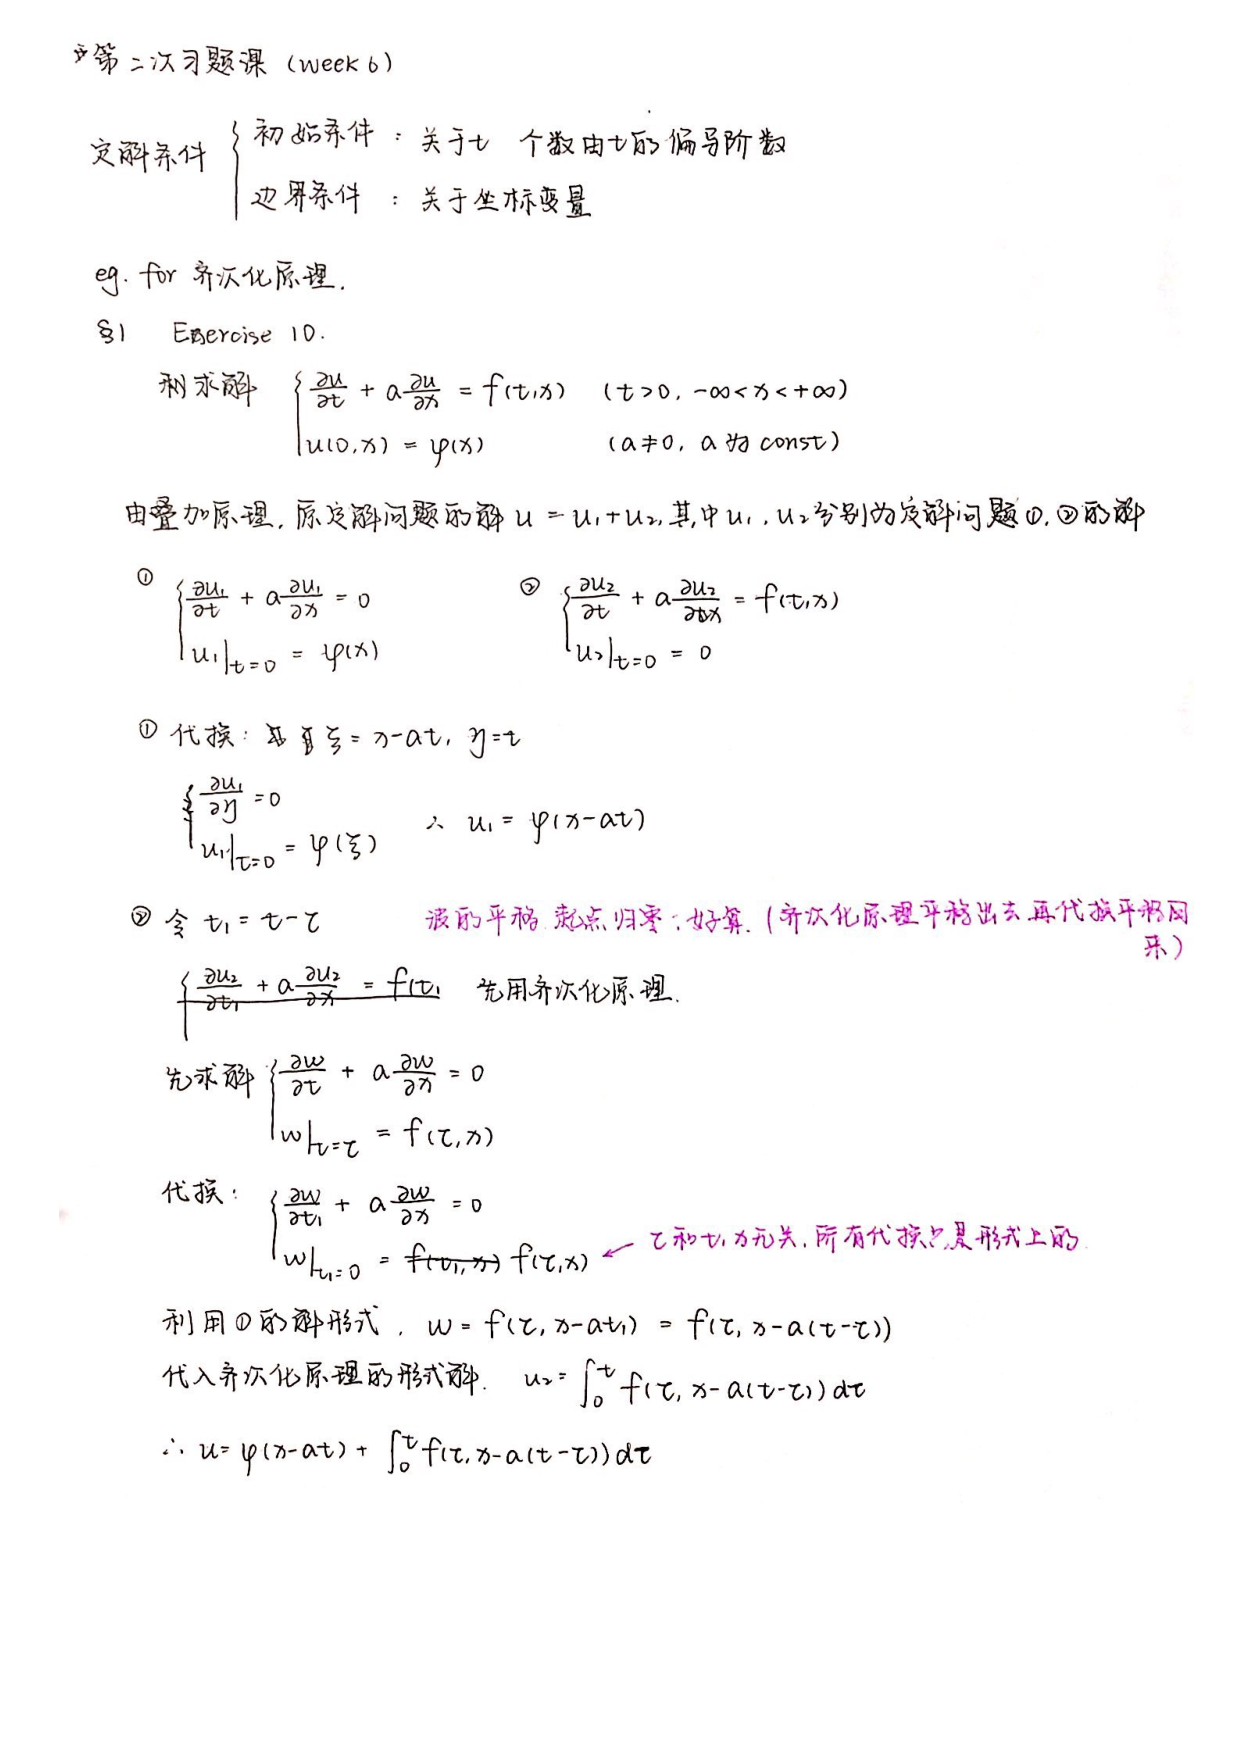
\includegraphics[scale=0.7]{ref_files/部分知识点的参考/齐次化原理.pdf}
		\newpage
		\paragraph{分离变量法}
		拆分变量之后,解固有值问题得到正交函数系,进一步得到通解(级数解),并利用定解条件得到特解。特殊情况包括在解固有值问题的时候,若ODE满足Bessel方程(柱坐标)或者Legendre方程(球坐标)的形式,则利用已有结论得到结果;以及非齐次情形,需要对定解条件以及泛定方程进行齐次化处理(注意顺序),\textit{具体方法见后面}
		\paragraph{积分变换法}
		积分变换法不需要考虑非齐次项,但是计算量emm...吾不言\newline
		积分变换法有一些points,比如边界条件 (Fourier变换没有) 是需要变换的,但是初始条件变换过去可以只先写一个$F[\varphi(M)]$,因为很有可能是在最后做反演变换的时候,乘起来变换回来卷积的时候就又回来了。
		\paragraph{基本解方法}
		基本解分为列出来基本解问题并求解,和代入积分式计算两部分。三种典型方程都有其对应的基本解模型,以及积分式计算公式。其中Poisson方程用Green函数求解,镜像法是在特殊的求解域下,用以对基本解求解的方法,故求出格林函数后只需代入积分公式即可。\par
		poisson方程(椭圆方程)、热传导方程(抛物方程)、弦振动方程(双曲方程)
		\subsection{掌握额外技能}
		数学物理方程不是孤立的一门课,而是和微积分课程一脉相承的,故在这门课程的计算中,会用到:\par
		\begin{enumerate}
			\item 解ODE(数学分析B1第六章)
			\item 欧拉方程(注意和Legendre方程区分,y前面的系数不一样)
			\item Fourier变换以及Fourier展开(数学分析B2第十二章)
			\item Laplace变换,反演变换以及各种性质(复变函数第七章)
			\item 留数定理及其计算(复变函数第五章)
			\item 对于方向导数的计算($\frac\partial{\partial n}$,在基本解方法的代入积分公式会用得到)
			\item 计算上用不到但是证明会用到的格林公式以及场论(数学分析B2第九章)
		\end{enumerate}\par
		还有这门课本身的一些例题上面的公式(如Legendre方程部分的$\displaystyle(m+n+1)\int_{0}^1x^mp_n(x)dx=m\int_0^1x^{m-1}p_{n-1}(x)dx$就出自例题。
	\section{关于一些方法}
		对于$\Delta_3u=0$之类的,求形如$u=u(r)$的解的问题,可以通过函数变换$u=v/r$来进行通解的求解。为使$u|_{r=0}$有限,应有$v(t,0)=0$
		\subsection{齐次化原理}
		不仅
		\subsection{特解法}
		用于处理方程非齐次的情形。不仅方程要变化,定解条件也要变化
		\subsection{解固有值问题}
		降阶法、特征根法、特殊函数法、欧拉方程(变量代换)、函数变换(有精力看一下)
		\subsection{特殊函数的积分求解}
		比如处理一个积分,积分项里面含有$P_\nu(x)$,积分域又恰好是Legendre函数的区间$(-1,1)$或$(1,1)$,其实可以想一下是不是可以通过转化方程,利用正交性来解题(有一个利用SL定理的概念)。不过很多题也会用到一些结论,比如Legendre部分的$\displaystyle\int_{-1}^1P_n(x)\,dx=0\quad(n\neq0)$。总的来说:\par
		\begin{enumerate}
			\item 积分区间,奇偶性
			\item 特殊结论(主要Legendre)、递推公式
			\item 固有函数(SL定理正交性)注意区间一定是方程的定义区间
		\end{enumerate}
		\subsection{正余弦变换}
		不建议用卷积公式,建议用定义
\end{document}
